\chapter{Monde et ses règles}
\section{Représentation et fonctionnement d'un monde}
\subsection{Définition d'un monde}
La structure du monde est imposé par le sujet : un tableau de dimension $\texttt{WIDTH} \times \texttt{HEIGHT}$. Il est constitué de nombres entiers positifs compris entre $0$ et $4294967295$ \footnote{Cet entier est la valeur maximale que peut prendre un entier positif (\lstinline{max unsigned_int}) en C} représentant l'état d'une cellule. A chaque élément du tableau est associé une couleur, également appelé état. Il existe une bijection entre le tableau d'un monde et sa représentation 2D comme on peut le voir sur la \autoref{fig:Conv_array_2D}. On a donc la relation suivante : $$i* WIDTH + j = k ,$$ k étant l'indice dans le tableau et $(i,j)$ les indices dans le monde 2D.

\begin{figure}[ht!]
    \centering
    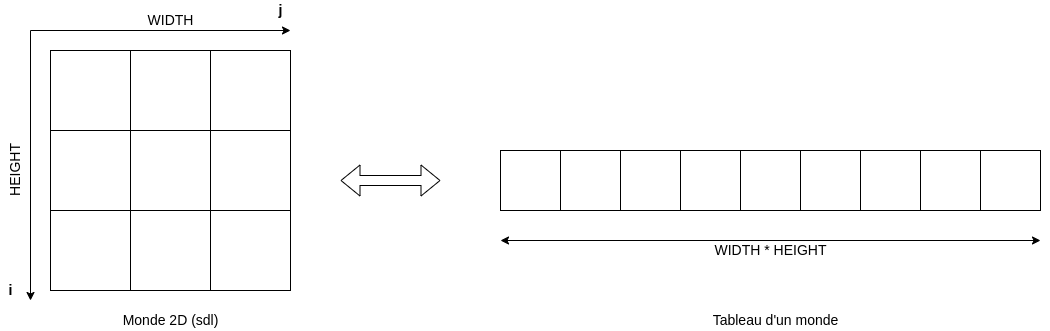
\includegraphics[width=0.95\textwidth]{"chap2/2D_to_Array.png"}
    \caption{Relation entre un tableau à une image de taille $\texttt{WIDTH}\times\texttt{HEIGHT}$}
    \label{fig:Conv_array_2D}
\end{figure}

Le monde est considéré comme un espace torique, c'est-à-dire que lorsqu'une cellule se déplace sur les bords de l'image, à l'image d'un planisphère \footnote{Les auteurs de ce rapport se sont essayés à l'antanaclase, ils espèrent avoir correctement appréhender le concept derrière cette figure de style}, la cellule se retrouve sur le bord opposé. Pour ce faire il a fallu implémenter une fonction \lstinline{int modulo(int x, int n)} complémentaire qui prenne en compte les nombres négatifs et qui retourne dans tous les cas un nombre positif.
\begin{lstlisting}
int modulo(int x, int n)
{
    if (x < 0) {
        return n + (x % n);
    } else
        return x % n;
}
\end{lstlisting}

Pour faire le lien entre la représentation sous forme de tableau d'un monde et sa représentation 2D, nous avons implémenté la fonction \lstinline{world_disp(struct world* w)}. Il a été nécessaire que le retour sur la sortie standard de la fonction soit compatible avec la librairie \texttt{sdl} afin de pouvoir afficher en couleur l'image (voir \autoref{fig:WorldDisplay}

\begin{figure}[ht]
    \centering
    \hspace*{\fill}
    \begin{subfigure}{0.15\textwidth}
        \centering
        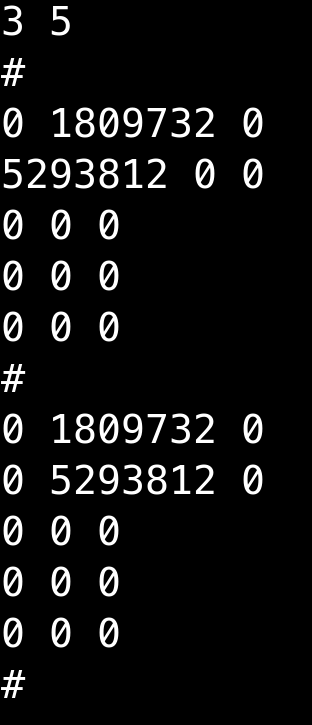
\includegraphics[width=\textwidth]{img/chap2/SortieStandard.png}
        \subcaption{Sortie Standard}
    \end{subfigure}
    \hfill
    \begin{subfigure}{0.15\textwidth}
        \centering
        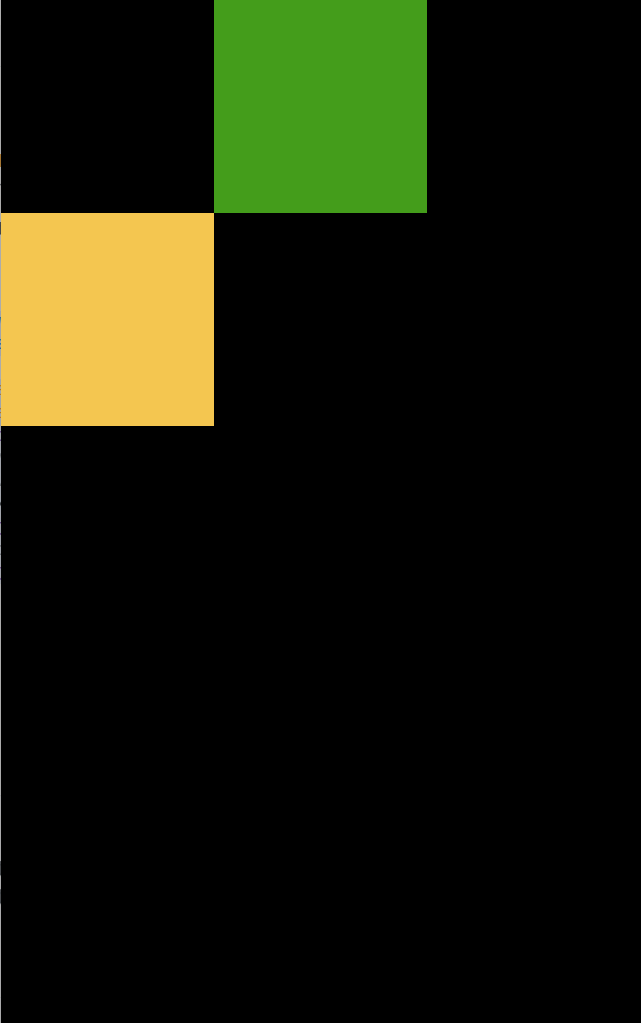
\includegraphics[width=\textwidth]{img/chap3/TestConflict1.png}
        \subcaption{Première image générée}
    \end{subfigure}
    \hfill
    \begin{subfigure}{0.15\textwidth}
        \centering
        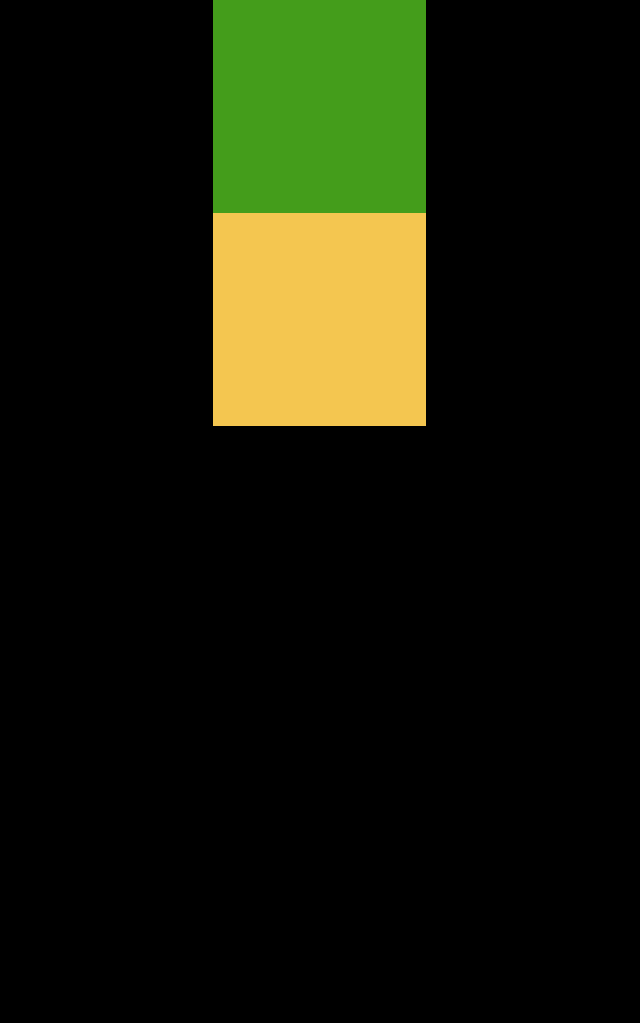
\includegraphics[width=\textwidth]{img/chap3/TestConflict2.png}
        \subcaption{Deuxième image générée}
    \end{subfigure}
    \hspace*{\fill}
    \caption{Sortie de \texttt{world\_display()} et résultat à l'affichage}
    \label{fig:WorldDisplay}
\end{figure}

\newpage
\subsection{Deux implémentations de monde}
\label{sec:ImplementationMonde}
Nous avons utilisé deux grandes catégories de mondes  lors de ce projet :
\begin{itemize}
    \item le monde du jeu de la vie (d'abord en noir et blanc puis en couleur) qui est généré de manière aléatoire (voir la \autoref{fig:jeu_de_la_vie});
    \item le monde du tas de sable représenté par la \autoref{fig:sablier}, (qui peut être ou ne pas être aléatoire).
\end{itemize}
\vspace{\parskip}

\begin{figure}[ht]
    \centering
    \hspace{\fill}
    \begin{subfigure}{0.35\textwidth}
        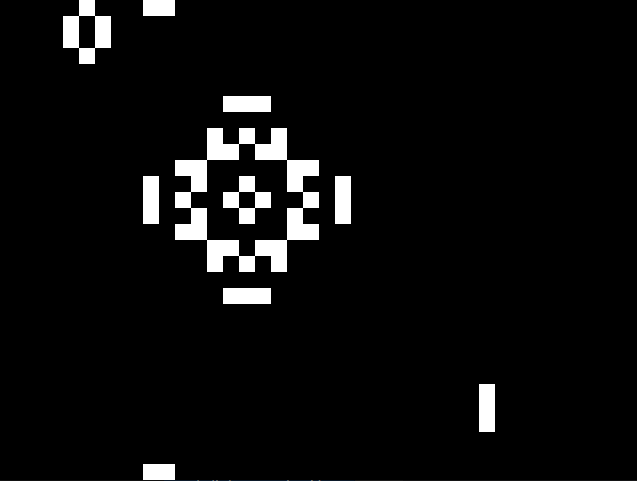
\includegraphics[width=\textwidth]{"chap2/jeu_de_la_vie.png"}
        \subcaption{Jeu de la vie}
        \label{fig:jeu_de_la_vie}
    \end{subfigure}
    \hfill
    \begin{subfigure}{0.35\textwidth}
        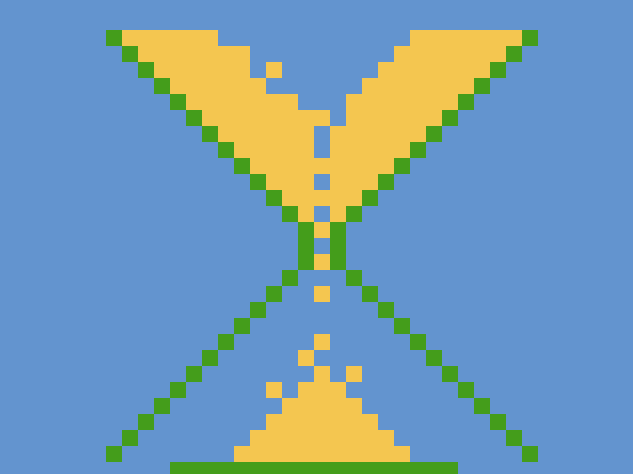
\includegraphics[width=\textwidth]{chap2/sablier.png}
        \subcaption{Sablier}
        \label{fig:sablier}
    \end{subfigure}
    \hspace{\fill}
    \caption{Image obtenue avec \texttt{SDL}}
    \label{fig:sdl_mondes}
\end{figure}

L'implémentation de ces deux mondes a mis en évidence deux types de comportements pour une cellule : le changement d'état lié à son entourage (jeu de la vie) et le déplacement d'une particule (sablier).

Nous avons regroupé les quelques couleurs primaires utilisées dans ce projet dans une énumération \lstinline{enum state}. Une couleur spéciale a été réservée sous le nom de \texttt{RANDOM\_COLOR} et à l'image de la carte \og 4 couleurs \fg{} dans un jeu de UNO, correspond de manière arbitraire à toutes les couleurs à la fois. Son utilisation est abordée plus en détaille dans la \autoref{sec:ReglesMotif}.

%Ces deux mondes ont utilisé des couleurs regroupées dans une structure appelée \texttt{state} : \texttt{DEAD} (noir), \texttt{ALIVE} (blanc), \texttt{EMPTY} (bleu), \texttt{GRASS} (vert), \texttt{SAND} (jaune) et une couleur spéciale appelée \texttt{RANDOM\_COLOR}.

Afin de générer un monde initial, nous avons utilisé une fonction \lstinline{struct world world_init(char opt, int seed)}. Comme explicité plutôt, il doit est possible de générer un monde aléatoire. Pour ce faire, lors du lancement de l'exécutable principal \texttt{project}, il est nécessaire d'ajouter l'option -s (option programmable grâce à la libairie \texttt{optget}) et d'ajouter à la suite un entier qui sera une graine à la génération pseudo-aléatoire du monde.

Une dernière fonction est disponible concernant les mondes, la fonction \lstinline{void world_apply_rule()} (manque ici les paramètres, pour des raisons visuelles). Elle permet d'appliquer les règles sur les cellules lorsque nécessaire. Cette fonction étant fortement liée à la façon dont nous résolvons les conflits, on en parle plus en détail dans la \autoref{sec:Conflits}.

Finalement, lors de la génération du monde, il est important de définir ce qu'est une cellule vide. En effet, toujours lors de la gestion des conflits, nous avons fait le choix de ne déplacer une cellule que lorsque l'endroit où elle veut se déplacer est vide. Or tout état est en réalité un entier. Nous avons fait le choix de prendre la valeur 0 pour définir une cellule vide, ce qui correspond à la valeur \texttt{DEAD} dans l'énumération de nos états.

\subsection{Tests concernant les mondes et complexité des fonctions} \label{sec:ReglesMotif}

On teste la génération d'un monde aléatoire, c'est-à-dire qu'on regarde si deux mondes généré aléatoirement sont bien différents. Pour ce faire, comme il y a une petite chance que deux mondes aléatoires soient identiques, on laisse la possibilité de régénéré un monde dix fois avec la même graine. Si au cours des 1O itérations, le premier monde est identique aux 10 autres avec des graines différentes, alors on considère que la génération d'un monde aléatoire n'est pas respectée.

La fonction \lstinline{void world\_apply\_rule()} étant intrinsèquement liée à la gestion des conflits et à de nombreux autres paramètres externes, elle est en réalité testée dans le fichier \texttt{test\_conflict.c}.

En ce qui concerne la complexité, si on pose $W$ la longueur et $H$ la largeur de l'image, on a:
\begin{itemize}
    \item \lstinline{world\_display}: on parcourt toutes les cases du monde et on les affiches donc la complexité est en $O(W\times H)$
    \item \lstinline{world\_init}: la complexité est de $O(W\times H)$ (car il faut associer à chaque cellule une valeur)
\end{itemize}

\section{Implémentation et évolution des règles par motifs}

Le principe d'un automate cellulaire est de définir des règles plus ou moins compliquées au début de l'algorithme et de les appliquer sur toutes les cellules du monde. Mais comment définir une règle ?

Une règle ne s'applique sur un pixel que dans des conditions spécifiques pré-établies. Nous nous sommes donc posez la question des cellules à observer, des conditions à remplir pour que la règle s'applique. Or dans le jeu de la vie, en plus de regarder l'état de la cellule à modifier, il faut également regarder ses cellules voisines. C'est pourquoi la première  implémentation des règles repose sur les informations suivantes :
\begin{itemize}
    \item un tableau de taille 9 (\lstinline{NB\_NEIGHBOUR}) contenant tous les voisins et la cellule a étudiée (située à l'indice 4 du tableau)
    \item un tableau qui contient les différentes modifications possibles (changements d'état ou déplacements) si la règle correspond à la situation du monde (la taille de ce tableau est déterminé par la valeur \lstinline{MAX\_STATE}) ;
    \item le nombre de changements possibles pour une règle
\end{itemize}
\vspace{\parskip}

Par soucis de clarté, nous avons fait le choix d'implémenter les changements à appliquer par une structure qui comprend:
\begin{itemize}
    \item la valeur de la cellule
    \item le déplacement selon \texttt{dx} et \texttt{dy}
\end{itemize}

Cette structure est la suivante dans notre code :
\begin{lstlisting}
    struct next_state {
        unsigned int next_color;
        int dx, dy;
    };
\end{lstlisting}
\vspace{\parskip}

\begin{figure}[h!]
    \centering
    \begin{subfigure}{0.75\textwidth}
        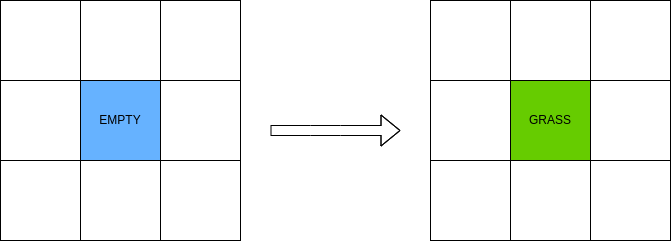
\includegraphics[width=\textwidth]{"chap2/change_couleur.png"}
        \subcaption{Changement de couleurs}
        \label{fig:chgt_color}
        \bigskip
    \end{subfigure}

    \begin{subfigure}{0.75\textwidth}
        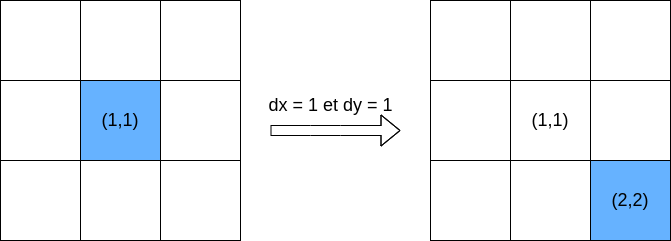
\includegraphics[width=\textwidth]{img/chap2/change_mov.png}
        \subcaption{Déplacement d'une particule}
        \label{fig:chgt_move}
    \end{subfigure}
    \caption{Les deux types de modifications pour une règle}
    \label{fig:modif_types}
\end{figure}

Nous avons choisi la convention suivante en ce qui concerne les changements d'une règle : soit on applique un déplacement, soit on applique un changement d'état. Le but de cette convention est de rester cohérent avec le principe de \bsc{Lavoisier} \footnote{En réalité, dans le jeu de la vie, des cellules naissent ou meurent, c-à-d des cellules apparaissent et disparaissent. Le principe physique précédent n'est donc pas respecté. Pour être plus juste, le principe de \bsc{Lavoisier} s'applique uniquement lorsqu'une cellule se déplace} - \emph{rien ne se perd, rien de ne crée, tout se transforme}. En effet, déplacer et modifier la couleur d'une cellule entre deux générations d'images revient à la faire disparaître.

Pour générer les règles de la vie, il a donc fallu générer tous les motifs possibles pour 9 voisins soit $2^9 = 512$ combinaisons. Nous nous sommes inspirés de l'écriture binaire pour générer tous les motifs en noir est blanc. L'inconvénient de cette méthode est qu'il correspond à la formule suivante: $$nombre\_couleurs^{nombre\_voisins} $$
En effet, plus le monde comporte d'états (ie plus il y a de couleurs), plus le nombre de motifs à générer est important. Il est également nécessaire de rappeler que la complexité de l'algorithme principal pour la génération d'une image dépend fortement du nombre de règles. En effet, pour chaque cellule l'algorithme cherche une règle compatible parmi toutes les règles existantes.

Une solution a été de faire des groupes de motifs en utilisant une couleur qui correspond à toutes les autres appelée \texttt{RANDOM\_COLOR} (définit dans la \autoref{sec:ImplementationMonde}). Cela à été fortement utile lors de l'implémentation de la chute de sable. Cependant, cette solution a un inconvénient. Lorsqu'on génère un motif on sait qu'il est unique. Cependant, plusieurs motifs avec des règles différentes peuvent être malencontreusement regroupés sous un même motif comportant \texttt{RANDOM\_COLOR}. En effet, en regardant le graphe \autoref{fig:motifs_avec_random}, si les cases blanches représentent cette couleur bonus, alors le motif 2 est un cas particulier du motif 1. En gagnant en complexité en diminuant le nombre de règle, on perd la bijection entre règle et motif.

\begin{figure}[ht]
    \centering
    \hspace*{\fill}
    \begin{subfigure}{0.3\textwidth}
        \centering
        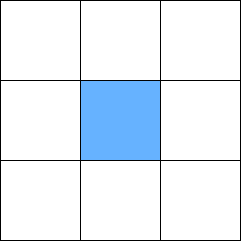
\includegraphics[width=\textwidth]{chap2/random_color1.png}
        \subcaption{Motif 1}
        \label{fig:motif2}
    \end{subfigure}
    \hfill
    \begin{subfigure}{0.3\textwidth}
        \centering
        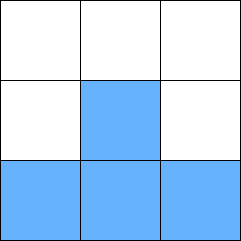
\includegraphics[width=\textwidth]{chap2/random_color2.png}
        \subcaption{Motif 2}
        \label{fig:motif1}
    \end{subfigure}
    \hspace*{\fill}
    \caption{Deux motifs : le motif (b) est inclus dans le motif (a)}
    \label{fig:motifs_avec_random}
\end{figure}

Il faut donc être prudent lors de l'implémentation des règles et de leur placement dans le tableau. En effet, c'est la première règle qui correspond qui est appliquée, les autres sont ignorées. Les règles les plus spécifiques doivent donc être en début du tableau et les plus génériques à la fin.

Cette solution n'est donc pas optimale de part sa forte complexité temporelle et sa fragilité. On doit ainsi trouver une autre manière de générer des règles, plus optimale, plus stable et surtout plus simple.

\section{Refonte des règles : des motifs aux fonctions}
\subsection{Limites des motifs}
On vient de voir que la forte complexité temporelle de la création des règles avec les motifs était un inconvénient majeur pour une bonne optimisation du projet. Mais encore, il ne semble pas intuitif d'utiliser des motifs avec certaines règles, par exemple du jeu de la vie. En effet, ce dernier ne comporte que deux règles :
\begin{itemize}
    \item Si une cellule morte est entourée par 3 cases vivantes, alors elle devient vivante
    \item Si une cellule vivante est entourée par moins d'une case vivante (isolement) ou par plus de quatre cases vivantes (surpopulation), alors elle meurt.
\end{itemize}
Il paraît donc plus naturel de chercher un moyen d'implémenter uniquement deux règles pour créer un jeu de la vie.
\subsection{Généricité des règles}
Une manière simple de représenter une règle est de le faire avec une fonction. En retournant un booléen, elle indique ainsi si elle doit être appliquée ou non. Dans l'exemple du jeu de la vie, on doit créer deux règles dans \texttt{rule.c}:
\begin{itemize}
    \item \lstinline{int born(const struct world* w, unsigned int i, unsigned int j)} pour vérifier si une cellule morte doit vivre ou pas ;
    \item \lstinline{int dead(const struct world* w, unsigned int i, unsigned int j)} pour vérifier si une cellule vivante doit mourir ou pas.
\end{itemize}

On doit alors modifier la structure d'une règle, en remplaçant le motif de la règle par un pointeur de fonction \lstinline{int (*match)(const struct world*, unsigned int, unsigned int)}, contenant dans le cadre du jeu de la vie une de ces fonctions.

La structure des règles devient alors :
\begin{lstlisting}
    struct rule {
        int (*match)(const struct world*, unsigned int, unsigned int);
        unsigned int len_changes;
        struct next_state next_state[MAX_STATE];
    };
\end{lstlisting}

Pour ce qui est des méthodes, seul la vérification de la correspondance des règles changent, puisqu'il n'est plus nécessaire de vérifier la superposition d'un motif mais simplement à exécuter la fonction pointée par l'attribut \lstinline{match} de la règle. \lstinline{rule_match()} devient alors :
\begin{lstlisting}
    int rule_match(const struct world* w, const struct rule* r, unsigned int i, unsigned int j)
    {   
        return r->match(w, i, j);
    }
\end{lstlisting}

\subsection{Avantages de la généricité des fonctions}
Améliorer les règles en passant d'une correspondance par motif à une vérification par exécution d'une fonction possède plusieurs avantages.

Le premier est la simplicité d'écriture des règles, puisqu'il est naturel de les imaginer avec une fonction. Ensuite, le cas du jeu de la vie montre qu'on obtient un gain non négligeable en espace (passage de $2^9$ à $2$ règles). En réalité, certaines règles sont plus sensibles que d'autres à ce gain. Par exemple, un monde régit par des règles de chute de sable (comme utilisé dans les \emph{achievements} 2 et 3) ne possède quasiment aucun gain avec la généricité des règles, ceux-ci étant imaginés comme pour une correspondance de motif. En revanche, une correspondance de motif reste quand même implémentable avec une fonction, ce que faisait d'ailleurs \lstinline{find_neighbours()} et \lstinline{compare_pattern ()}dans \lstinline{rule_match}.

Enfin, on réalise que l'utilisation d'une structure abstraite dans l'en-tête facilite grandement cette transition, puisqu'il a été aisé de faire cette transition sans devoir modifier le projet principal.